\documentclass{beamer}
\usepackage{framed}
\usepackage{graphicx}

\begin{document}
\section{Integer Programming}
\subsection{Canonical Form}
%================================================ %
\begin{frame}
	\frametitle{Canonical Form}
\begin{figure}
\centering
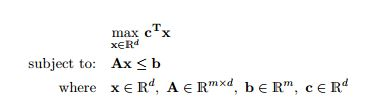
\includegraphics[width=0.7\linewidth]{canonical}

\end{figure}
\begin{itemize}
\item The feasible region, is defined by the set of inequalities $Ax \leq b$. In two
dimensions, i.e. if d = 2, this problem can be represented and solved graphically as polyhedron in the Euclidean plane.
\item  The idea
is to represent the cost vector c as a level set in the plane. 
\item Then, moving this level set
towards the highest possible value so that still intersects our feasible region, i.e. the polyhedron
P defined by A, yields the optimal solution.
\end{itemize}

\end{frame}

%================================================ %
\subsection{LP Divisibility}
\begin{frame}
\frametitle{Divisibility}	
\begin{itemize}
\item Divisibility is one of the conventional LP assumptions.
\item Divisibility allowed us to consider activities in fractions: We could produce 7.8 units of a product,
buy 12500.33 liters of oil, hire 12.123 people for full time, etc. 
\item Divisibility assumption is very defensible at
times but not always. 
\item We can easily buy 12500.33 liters of oil but can not employ 12.123 people. 
\end{itemize}
\end{frame}

%================================================= %
\begin{frame}
\frametitle{Divisibility}
\begin{itemize}
\item Clearly
some activities cannot be done in fractions and must be specified in integers for implementation.
\item As soon as
 some of the activities are set to be integers, we are in \textbf{Integer Programming} domain. 
 \item Formally, in an integer
 program some decision variables are forced to be integers.
\end{itemize}
\end{frame}
%================================================== %
\subsection{Lattice Point}
\begin{frame}
	\begin{figure}
\centering
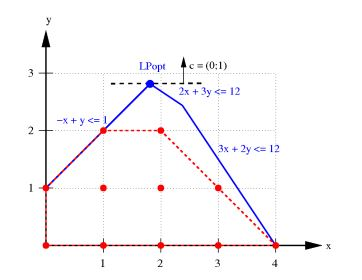
\includegraphics[width=0.7\linewidth]{LatticePoints}
\caption{}
\label{fig:LatticePoints}
\end{figure}

\end{frame}
\subsection{Example of IP Problem}
\begin{frame}
\frametitle{IP Example:  Tables and Chairs}
\begin{itemize}
	\item Suppose we consider producing chairs and tables using only 21 $m^2$ of
	wood. Each chair (table) requires 6 (7) $m^2$ of wood. 
	\item Each chair is sold at $\$12$ (×10) and each table is sold
	at $\$13$ ($\times 10$). 
	\item Let C and T denote the number of tables and chairs produced. 
	\item The IP formulation below
	maximizes the revenue:
\end{itemize}
\end{frame}
%======================================================================== %
\begin{frame}
\frametitle{IP Example:  Tables and Chairs}
\begin{figure}
\centering
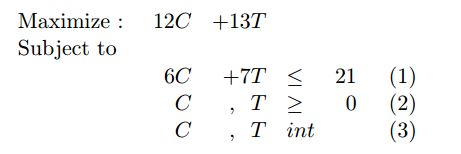
\includegraphics[width=0.7\linewidth]{IPintro1}
\end{figure}

\end{frame}
%============================================================================== %
\begin{frame}
\frametitle{IP Example:  Tables and Chairs}
\begin{figure}
\centering
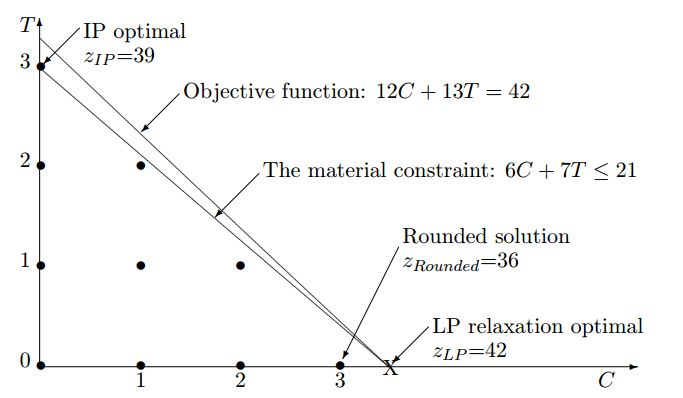
\includegraphics[width=0.7\linewidth]{IPintro2}

\end{figure}
\end{frame}
%================================================ %
\subsection{LP Relaxation}
\begin{frame}
\frametitle{LP Relaxation}
\large
\begin{itemize}
\item 
Solving an IP can be as straightforward as solving the associated LP
and rounding the solution, but only in some cases. (i.e. by coincidence rather than by definition)
\item To understand what can wrong with this approach, we will first solve the IP
removing constraint and round down  the optimal values of C and T to satisfy
the integer constraint. 
\item (Question: why not to round up?)
\item When the integer constraints are removed from an IP formulation, we obtain an LP formulation. This
LP formulation is called the \textbf{LP relaxation}.
\end{itemize}
\end{frame}
%======================================================= %
\begin{frame}
	\frametitle{LP Relaxation}
	\begin{itemize}
\item LP solution is (7/2,0) and is not integer so we round it down to (3,0). 
\item The objective value at (3,0) is
36. 
\item The optimal solution to IP is (0,3) with the objective value 39. 
\item 3 units of difference between objective
value of the IP optimal and the rounded solution can be significantly higher in more complex problems.
\item As
a summary we cannot use rounded solutions of LP relaxations.
	\end{itemize}
\end{frame}
%======================================================= %
\begin{frame}
\frametitle{LP Relaxation}
\begin{itemize}
\item Given an integer program (IP), there is an associated lenear program (LR)
called the \textbf{linear relaxation}. 
\item It is formed by dropping (relaxing) the integrality
restrictions. 
\item Since (LR) is less constrained than (IP), the following are immediate:
\end{itemize}

\end{frame}
%======================================================= %
\begin{frame}
	\frametitle{LP Relaxation}
\begin{itemize}
\item[1] If (IP) is a minimization problem, the optimal objective value of (LR) is
less than or equal to the optimal objective value of (IP).
\item[2] If (IP) is a maximization problem, the optimal objective value of (LR) is
greater than or equal to the optimal objective value of (IP),
\item[3] If (LR) is infeasible, then so is (IP).
\item[4] If all the variables in an optimal solution of (LR) are integer-valued, then
that solution is optimal for (IP) too.
\end{itemize}
\end{frame}
\begin{frame} 
\begin{itemize}
\item[5] If the objective function coefficients are integer-valued, then for minimization
	problems, the optimal objective value of (IP) is greater than
	or equal to the ceiling of the optimal objective value of (LR). For maximization
	problems, the optimal objective value of (IP) is less than or
	equal to the floor of the optimal objective value of (LR). 
\end{itemize}
\end{frame}
%=============== %
\subsection{Solution Techniques}
\begin{frame}
\begin{itemize}
\item For simple problems one
	can evaluate all the integer solutions in the feasible region and pick the best. 
\item However, for real problems
	this approach will take practically infinite amount of time. 
\item The solution procedures for IP’s are still under
	development. 
\item Two approaches are common: Branch and Bound technique, and Cutting planes. 
\item Cutting Planes are outside the scope of our module.
\end{itemize}

\end{frame}
%======================================================= %
\subsection{Divide and Conquer}
\begin{frame}
	\Large
	\noindent \textbf{Divide and Conquer}
	\begin{figure}
		\centering
		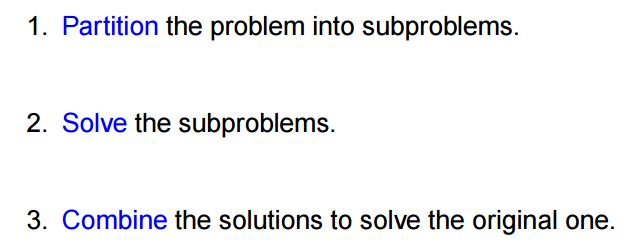
\includegraphics[width=0.9\linewidth]{divideandconquer}
		
	\end{figure}
	
\end{frame}
%==========================================================
\begin{frame}
	\frametitle{Branch-and-bound}
	%= http://web.mit.edu/15.053/www/AMP-Chapter-09.pdf
\noindent \textbf{Branch-and-bound}
	\begin{itemize}
		\item Branch-and-bound is essentially a strategy of ‘‘divide and conquer.’’ The idea is to partition the feasible
		region into more manageable subdivisions and then, if required, to further partition the subdivisions. 
		\item In
		general, there are a number of ways to divide the feasible region, and as a consequence there are a number of
		branch-and-bound algorithms. 
		
%		\item We shall consider one such technique, for problems with only binary variables,
%		in Section 9.7. 
		\item For historical reasons, the technique that will be described next usually is referred to as the
		branch-and-bound procedure.
		
	\end{itemize}
	
\end{frame}
%======================================================= %


%======================================================= %
\subsection{Enumeration Tree}
\begin{frame}
	\frametitle{Enumeration Tree}
	\begin{figure}
		\centering
		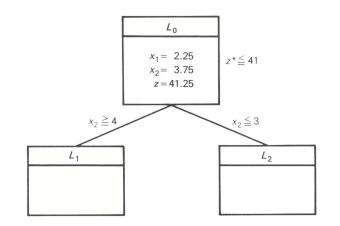
\includegraphics[width=0.7\linewidth]{enumerationtree1}
		\caption{}
		\label{fig:enumerationtree1}
	\end{figure}
	
\end{frame}
\begin{frame}
	\frametitle{Enumeration Tree}
	\begin{figure}
		\centering
		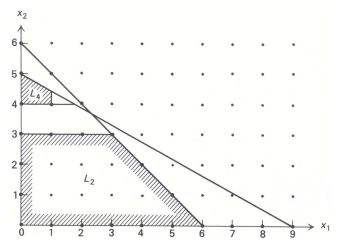
\includegraphics[width=0.7\linewidth]{enumerationtree2}
		\caption{}
		\label{fig:enumerationtree2}
	\end{figure}
	
\end{frame}
%================================================ %
\subsection{Difficulties of Integer Programming}
% % - http://www.inf.ufpr.br/aurora/disciplinas/topicosia2/livros/search/integer.pdf
\begin{frame}
	\begin{itemize}
		\item It is not always the case that branch and bound quickly
		solves integer programs.
		
		\item In particular, it is possible that the bounding aspects
		of branch and bound are not invoked, and the branch and bound algorithm can
		then generate a huge number of subproblems. 
		\item In the worst case, a problem
		with n binary variables (variables that have to take on the value 0 or 1) can
		have $2^n$ subproblems. 
		\item This exponential growth is inherent in any algorithm for
		integer programming, 
	\end{itemize}
	
\end{frame}
%======================================================= %
\subsection{Branch and Bound}
\begin{frame}
	\frametitle{Branch and Bound}
	\Large
	\begin{figure}
		\centering
		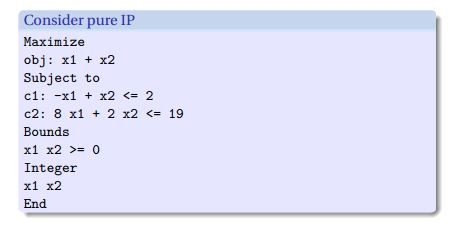
\includegraphics[width=1.1\linewidth]{BranchBound1}
	\end{figure}
	
\end{frame}
\begin{frame}
	\frametitle{Branch and Bound}
	\Large
	\begin{figure}
		\centering
		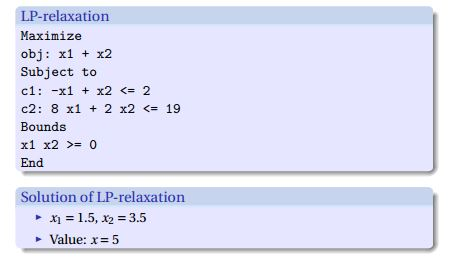
\includegraphics[width=1.1\linewidth]{BranchBound2}
	\end{figure}
	
\end{frame}
\begin{frame}
	\frametitle{Branch and Bound}
	\Large
	\begin{figure}
		\centering
		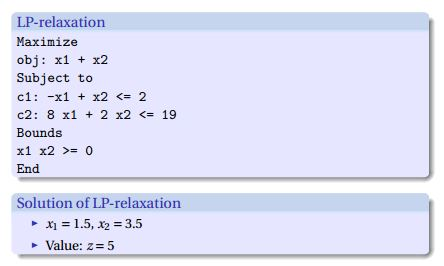
\includegraphics[width=1.1\linewidth]{BranchBound3}
	\end{figure}
	
\end{frame}
\begin{frame}
	\frametitle{Branch and Bound}
	\Large
	\begin{figure}
		\centering
		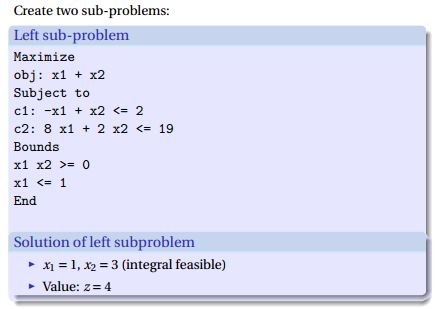
\includegraphics[width=1.1\linewidth]{BranchBound4}
	\end{figure}
	
\end{frame}
\begin{frame}
	\frametitle{Branch and Bound}
	\Large
	\begin{figure}
		\centering
		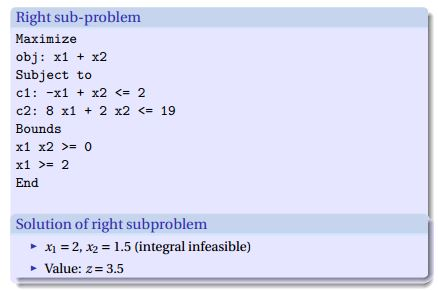
\includegraphics[width=1.1\linewidth]{BranchBound5}
	\end{figure}
	
\end{frame}
\begin{frame}
	\frametitle{Branch and Bound}
	\Large
	\begin{figure}
		\centering
		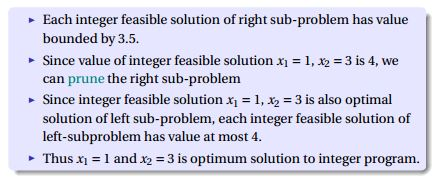
\includegraphics[width=1.1\linewidth]{BranchBound6}
	\end{figure}
	
\end{frame}
%=============================================== %
\end{document}